\documentclass[12pt,a4paper]{article}


\usepackage[in, plain]{fullpage}
\usepackage{array}
\usepackage{../../../pas-math}

%-------------------------------------------------------------------------------
%          -Packages nécessaires pour écrire en Français et en UTF8-
%-------------------------------------------------------------------------------
\usepackage[utf8]{inputenc}
\usepackage[frenchb]{babel}
\usepackage[T1]{fontenc}
\usepackage{lmodern}
\usepackage{textcomp}



%-------------------------------------------------------------------------------

%-------------------------------------------------------------------------------
%                          -Outils de mise en forme-
%-------------------------------------------------------------------------------
\usepackage{hyperref}
\hypersetup{pdfstartview=XYZ}
%\usepackage{enumerate}
\usepackage{graphicx}
\usepackage{multicol}
\usepackage{tabularx}
\usepackage{multirow}


\usepackage{anysize} %%pour pouvoir mettre les marges qu'on veut
%\marginsize{2.5cm}{2.5cm}{2.5cm}{2.5cm}

\usepackage{indentfirst} %%pour que les premier paragraphes soient aussi indentés
\usepackage{verbatim}
\usepackage{enumitem}
\usepackage[usenames,dvipsnames,svgnames,table]{xcolor}

\usepackage{variations}

%-------------------------------------------------------------------------------


%-------------------------------------------------------------------------------
%                  -Nécessaires pour écrire des mathématiques-
%-------------------------------------------------------------------------------
\usepackage{amsfonts}
\usepackage{amssymb}
\usepackage{amsmath}
\usepackage{amsthm}
\usepackage{tikz}
\usepackage{xlop}
%-------------------------------------------------------------------------------



%-------------------------------------------------------------------------------


%-------------------------------------------------------------------------------
%                    - Mise en forme avancée
%-------------------------------------------------------------------------------

\usepackage{ifthen}
\usepackage{ifmtarg}


\newcommand{\ifTrue}[2]{\ifthenelse{\equal{#1}{true}}{#2}{$\qquad \qquad$}}

%-------------------------------------------------------------------------------

%-------------------------------------------------------------------------------
%                     -Mise en forme d'exercices-
%-------------------------------------------------------------------------------
%\newtheoremstyle{exostyle}
%{\topsep}% espace avant
%{\topsep}% espace apres
%{}% Police utilisee par le style de thm
%{}% Indentation (vide = aucune, \parindent = indentation paragraphe)
%{\bfseries}% Police du titre de thm
%{.}% Signe de ponctuation apres le titre du thm
%{ }% Espace apres le titre du thm (\newline = linebreak)
%{\thmname{#1}\thmnumber{ #2}\thmnote{. \normalfont{\textit{#3}}}}% composants du titre du thm : \thmname = nom du thm, \thmnumber = numéro du thm, \thmnote = sous-titre du thm

%\theoremstyle{exostyle}
%\newtheorem{exercice}{Exercice}
%
%\newenvironment{questions}{
%\begin{enumerate}[\hspace{12pt}\bfseries\itshape a.]}{\end{enumerate}
%} %mettre un 1 à la place du a si on veut des numéros au lieu de lettres pour les questions 
%-------------------------------------------------------------------------------

%-------------------------------------------------------------------------------
%                    - Mise en forme de tableaux -
%-------------------------------------------------------------------------------

\renewcommand{\arraystretch}{1.7}

\setlength{\tabcolsep}{1.2cm}

%-------------------------------------------------------------------------------



%-------------------------------------------------------------------------------
%                    - Racourcis d'écriture -
%-------------------------------------------------------------------------------

% Angles orientés (couples de vecteurs)
\newcommand{\aopp}[2]{(\vec{#1}, \vec{#2})} %Les deuc vecteurs sont positifs
\newcommand{\aopn}[2]{(\vec{#1}, -\vec{#2})} %Le second vecteur est négatif
\newcommand{\aonp}[2]{(-\vec{#1}, \vec{#2})} %Le premier vecteur est négatif
\newcommand{\aonn}[2]{(-\vec{#1}, -\vec{#2})} %Les deux vecteurs sont négatifs

%Ensembles mathématiques
\newcommand{\naturels}{\mathbb{N}} %Nombres naturels
\newcommand{\relatifs}{\mathbb{Z}} %Nombres relatifs
\newcommand{\rationnels}{\mathbb{Q}} %Nombres rationnels
\newcommand{\reels}{\mathbb{R}} %Nombres réels
\newcommand{\complexes}{\mathbb{C}} %Nombres complexes


%Intégration des parenthèses aux cosinus
\newcommand{\cosP}[1]{\cos\left(#1\right)}
\newcommand{\sinP}[1]{\sin\left(#1\right)}


%Probas stats
\newcommand{\stat}{statistique}
\newcommand{\stats}{statistiques}
%-------------------------------------------------------------------------------

%-------------------------------------------------------------------------------
%                    - Mise en page -
%-------------------------------------------------------------------------------

\newcommand{\twoCol}[1]{\begin{multicols}{2}#1\end{multicols}}


\setenumerate[1]{font=\bfseries,label=\textit{\alph*})}
\setenumerate[2]{font=\bfseries,label=\arabic*)}


%-------------------------------------------------------------------------------
%                    - Elements cours -
%-------------------------------------------------------------------------------




\title{Correction des de la feuille 2 sur les angles}
\date{}


\graphicspath{{./img/}}
\begin{document}
	
\maketitle

\vspace*{-1cm}

\section*{Exercice 17}

Je sais que les droites, $(AL)$ et $(TO)$ sont parallèles et les angles $\widehat{ALT}$ et $\widehat{LTO}$ sont alternes-internes.
Or si deux droites coupées par une sécante sont parallèles, alors les angles alternes-internes ont la même mesure.
Donc l'angle $\widehat{LTO}$ mesure 97\degree .


\section*{Exercice 18}

\begin{center}
	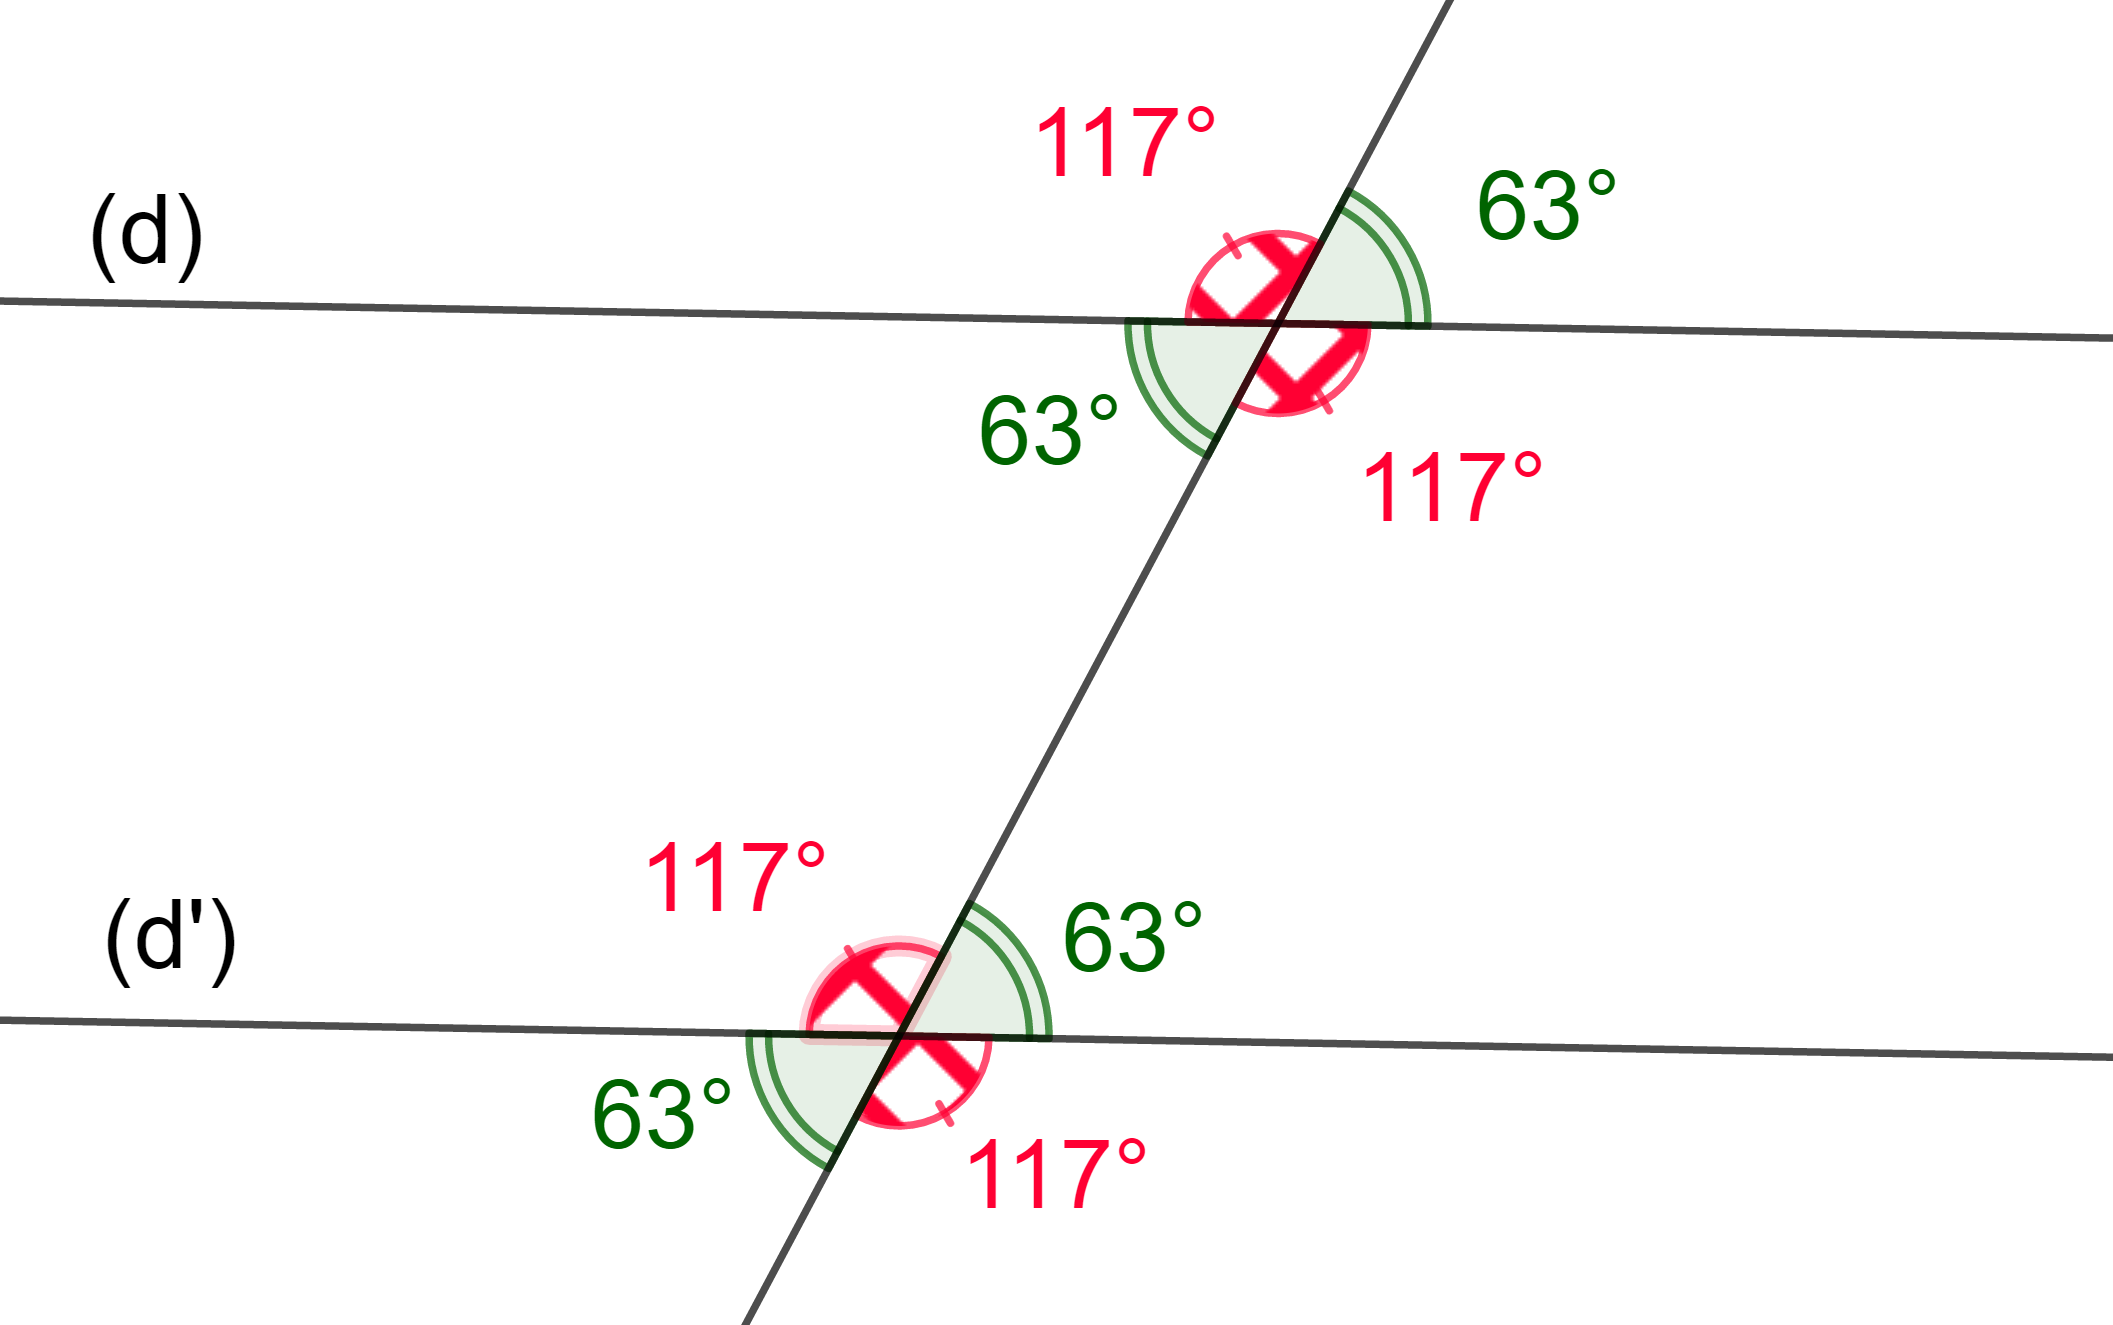
\includegraphics[scale=0.15]{ex18}
\end{center}


\section*{Exercice 16}

\begin{enumerate}[label=\alph*.]
	\item Les angles $\widehat{xMu}$ et $\widehat{vMy}$ sont opposés par le sommet, ils ont la même mesure. Donc l'angle $\widehat{vMy}$ mesure 125\degree .
	
	
	\item Les droites $(xy)$ et $(zf)$ sont parallèles et les angles $\widehat{vMy}$ et $\widehat{zNu}$ sont alternes-internes, ils ont la même mesure. Donc l'angle  $\widehat{zNu}$ mesure 125\degree .
	
	Les droites $(xy)$ et $(zf)$ sont parallèles et$\widehat{vMy}$ et $\widehat{vNt}$ sont correspondants, ils ont la même mesure. Donc l'angle  $\widehat{vNt}$ mesure 125\degree .
	Les angles 
\end{enumerate}

\newpage

\section*{Exercice 21}


Les droites $(AB)$ et $(CD)$ sont parallèles et les angles $\widehat{BRS}$ et $\widehat{CSR}$ sont alternes-internes, ils ont la même mesure. Donc l'angle $\widehat{CSR}$ mesure 20\degree .\\


On a $\widehat{RST}$ = 57\degree et $\widehat{CSR}$ = 20\degree . Donc l'angle $\widehat{CST}$ mesure 37\degree  (57\degree  - 20\degree ).\\


Les droites $(EF)$ et $(CD)$ sont parallèles et les angles $\widehat{STF}$ et $\widehat{CST}$ sont alternes-internes, ils ont la même mesure. Donc l'angle $\widehat{CSR}$ mesure 37\degree .


\section*{Exercice 25}

\begin{enumerate}[label=\alph*.]
	\item $\widehat{LOP}$ est un angle plat. Donc $\widehat{LON}$ = 180\degree  - 128\degree = 52\degree .
	
	\item
	
	%\begin{multicols}{2}
		Dans le triangle LON, la somme des mesure des angles est égale à 180\degree . Donc $\widehat{ONL}$ = 180\degree  - (43\degree  +  52\degree ) = 85\degree .
		
		\begin{center}
			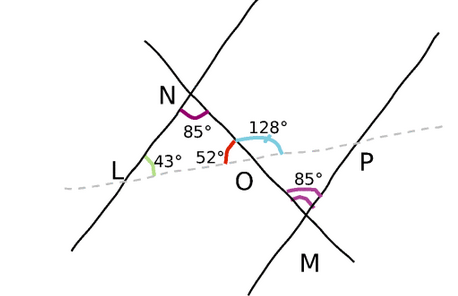
\includegraphics[scale=0.7]{ex25_1}
		\end{center}
	%\end{multicols}
	
	\item Les angles $\widehat{ONL}$ et $\widehat{OMP}$ sont alternes-internes et de même mesure, donc $(LN)$ et $(MP)$ sont parallèles.
	
	
	\item \ 
	\begin{center}
		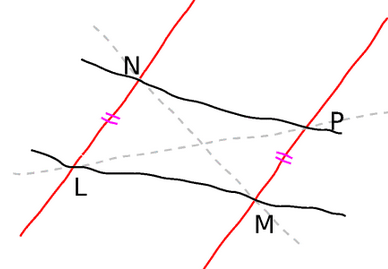
\includegraphics[scale=0.6]{ex25_2}
	\end{center}

	Je sais que $(LN)$ est parallèles $(MP)$  et que $LN = MP$.
	Or si un quadrilatère non croisé a deux cotés opposés parallèles et de même mesure alors c'est un parallélogramme.
	Donc le quadrilatère LNPM est un parallélogramme.
	 
\end{enumerate}
\end{document}